\chapter{Optimizing Code Generated by Iconc}

Author: Anthony Jones

Since Ken Walker produced iconc, several optimizations have been
implemented with the goal of improving execution time of the generated
executable. The goals of these optimizations are to make the
intermediate code as small as possible and to speed up the resulting
executable. First a brief summary of the internal representation of
the C code is provided. This is necessary because most of these
optimizations rely heavily on analyzing the internal C code. Following
this, the individual optimizations are discussed in detail.

There are different levels at which compiler optimizations may be
performed. One level of optimization deals with the front end and
intermediate code generation. Some examples of these optimizations
include common subexpression elimination, copy propagation, dead-code
elimination, constant folding, loop unrolling, and strength reduction.
Another level of optimization is machine specific, including efficient
register assignments, use of platform-specific instructions that offer
greater performance, or doing peephole transformations [ASU86]. The
optimizations implemented thusfar for the Icon compiler are not
platform-specific because iconc translates Icon code into C code which
then calls the native C compiler to finish the job.



\section{Areas Where Iconc Can Be Improved}

Iconc's compiled code is often many times faster than VM-interpreted
code, but is far from optimal. The next few sections describe
components of the existing compiler that were optimized by Anthony
Jones and are now part of the Unicon language distribution.

An examination of Icon's generated intermediate C code suggested many
areas of improvement. Some of the optimizations possible were
eliminating redundant system calls, replacing Icon literals with C
literals, and eliminating unnecessary logic in variable initialization
blocks.

\subsection{Redundant Function Calls}

A macro named \texttt{Poll()} is called every so often to handle
certain system operations such as processing window system events. The
iconc compiler initially did a naive job of placing these function
calls in the generated code. Often there were two calls to
\texttt{Poll()} one right after the other or only a simple assignment
between two calls. The objective of this optimization is to remove the
redundancy and let a reasonable number of calls remain.

\subsection{Constant Propagation}

Simple literals appearing in source programs are assigned into the
local variable descriptor table within a procedure. This descriptor
table is an array of complicated structures and pointers that incurs
many memory references simply for a constant. It is doubtful that most
C compilers would recognize these values as constants and
propagate them accordingly. The objective is to remove assignments of
constants into the descriptor table and replace references to those
descriptor locations with constant values.

\subsection{Variable Initialization}

At the beginning of every intermediate procedure there are several
loops that initialize local variables and parameters.  Sometimes these
loops initialize only one or two variables. In certain situations the
loop will not be executed at all, but the code for the loop is still
generated, requiring a comparison when the program executes. The
object of this part is to simplify the initialization loops and to
remove loops that have no effect.

\section{Enabling Optimizations}

All the changes made to the Icon compiler in order to implement these
optimizations were done with C compiler directives so that each
optimization can be turned on or off during compilation.

All directives are included in \textfn{src/c/define.h}. The symbols
\texttt{OptimizePoll}, \texttt{OptimizeLit}, and \texttt{OptimizeLoop}
turn on redundant \texttt{Poll()} removal,
literal propagation, and loop optimizations respectively.

An additional symbol, \texttt{LoopThreshold} has a default value of
7. This constant, used in the loop unrolling optimizations, is a limit
on the number of entries that may be unrolled in variable
initialization loops.


\section{Intermediate Code Representation}

This section briefly describes how the intermediate C code is
represented and generated internally by the Icon compiler.  The
majority of the functions that generate this internal representation
and print it to a file are contained in the following compiler source
files: \textfn{ccode.c}, \textfn{codegen.c}, and \textfn{inline.c}.

\subsection{How Code is Generated}

Once the source code is parsed and evaluated, the intermediate C code
needs to be generated and output to a file for compilation by the
native C compiler. First the compiler builds a syntax tree plus symbol
tables and other necessary structures. Then, the header file is
created. This includes standard definitions necessary for all Icon
programs and structures and variables specific to the program being
compiled. Next, the \texttt{proccode} function is called for each
function in the tree. This outputs the function definition and
variable in initialization code, and then steps through the syntax
tree and creates C code to represent the body of the function. After
all the code for the body of the current procedure is generated
internally, the code is then written to the file.

The internal C code is represented through a C structure called
\texttt{struct code} which is shown below.

\goodbreak
\begin{iconcode}
struct code \{\\
\>int cd\_id;\\
\>struct code *next;\\
\>struct code *prev;\\
\>union \ cd\_fld \ fld[1];\\
\};\\
\end{iconcode}


The \texttt{cd\_id} field is an identifier signaling what type of code
is held in this structure. This field may be set to one of the
following enumerated values. Each value corresponds to a type of code
that can be written to the intermediate C code. The table in Figure
25-1 contains the enumerated name along with its integer value and a
short description.

\begin{center}
\tablefirsthead{\hline
{\itshape Code Type} &
{\itshape Value} &
{\itshape Description}\\}
\tablehead{\hline
{\itshape Code Type} &
{\itshape Value} &
{\itshape Description}\\}
\tabletail{}
\tablelasttail{}
\begin{xtabular}{|>{\texttt\bgroup}m{1in}<{\egroup}|m{0.5in}|m{2.5in}|}
\hline
C\_Null &
\raggedleft 0 &
 No code in this struct\\\hline
C\_CallSig &
\raggedleft 1 &
 Call a signal (function)\\\hline
 C\_RetSig &
\raggedleft 2 &
 Return a signal\\\hline
 C\_NamedVar &
\raggedleft 3 &
 Reference a variable\\\hline
 C\_Goto &
\raggedleft 4 &
 Goto statement\\\hline
 C\_Label &
\raggedleft 5 &
 Label statement\\\hline
 C\_Lit &
\raggedleft 6 &
 Literal value\\\hline
 C\_Resume &
\raggedleft 7 &
 Resume signal\\\hline
 C\_Continue &
\raggedleft 8 &
 Continue signal\\\hline
 C\_FallThru &
\raggedleft 9 &
 Fall through signal\\\hline
 C\_PFail &
\raggedleft 10 &
 Procedure failure\\\hline
 C\_PRet &
\raggedleft 11 &
 Procedure return\\\hline
 C\_PSusp &
\raggedleft 12 &
 Procedure suspend\\\hline
 C\_Break &
\raggedleft 13 &
 Break out of signal handling switch\\\hline
 C\_LBrack &
\raggedleft 14 &
 Start of a new C block\\\hline
 C\_RBrack &
\raggedleft 15 &
 End of a C block\\\hline
 C\_Create &
\raggedleft 16 &
 Call create() for a create expression\\\hline
 C\_If &
\raggedleft 17 &
 If statement\\\hline
 C\_SrcLoc &
\raggedleft 18 &
 Source file name\\\hline
 C\_CdAry &
\raggedleft 19 &
 Array of code pieces\\\hline
\end{xtabular}
\end{center}
{\centering\selectlanguage{english}
Figure 25-1: Code Types
\par}


The \texttt{fld} field is important and is directly linked to what
type of code the \texttt{struct code} is defined as.  For example, if
a \texttt{struct code} is defined as \texttt{C\_If} then
\texttt{fld[0]} is a pointer to another \texttt{struct code} that
corresponds to the if portion of the statement, and \texttt{fld[1]} is
another pointer to a \texttt{struct code} representing the then
portion of the statement. In fact there are two macros for extracting
each pointer. These macros plus macros for all the other code types
are found in the \texttt{ccode.h} header file. However, there is one
special case that requires some explanation. If the \texttt{cd\_id} is
\texttt{C\_CdAry} then the \texttt{fld} element is an unspecified
length of \texttt{cd\_fld} unions. In this case all even indices into
the array are tags describing the contents of the following array
element. There is a special marker, \texttt{A\_End}, that signifies
the end of the array.

Figure 25-2 shows
these field identifiers along with their corresponding fields for an
assignment statement.

\begin{center}
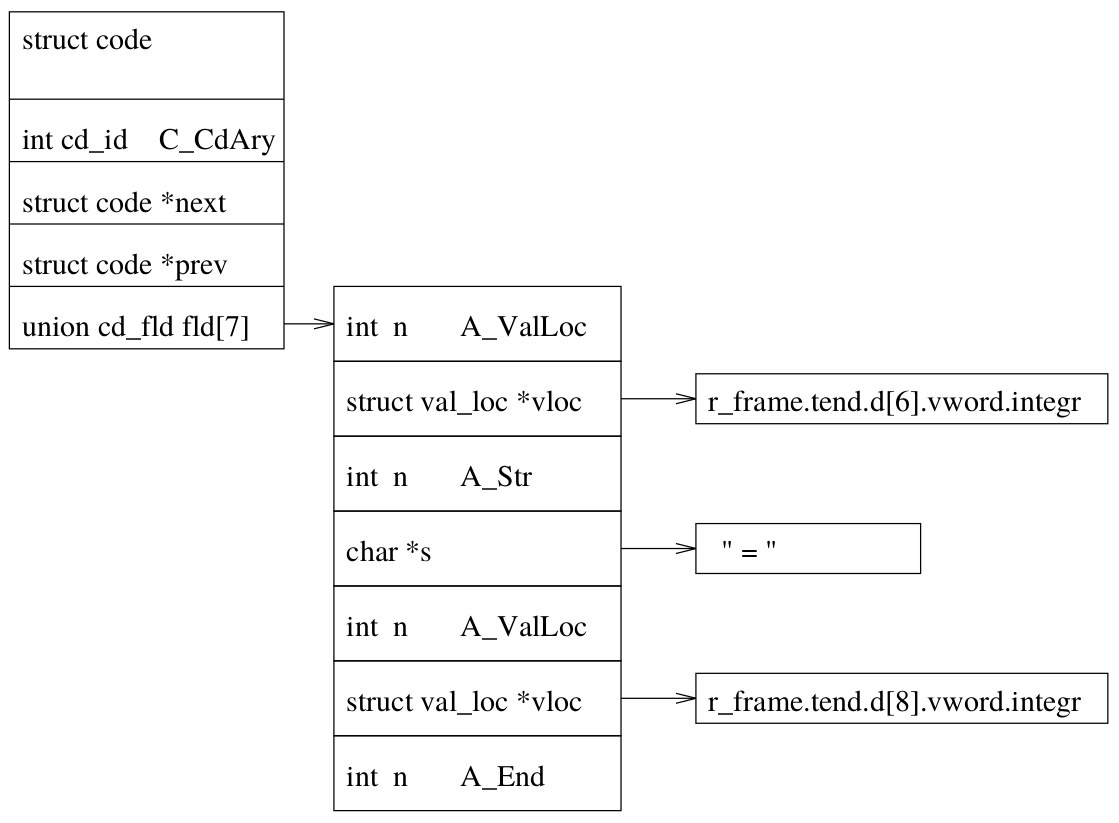
\includegraphics[width=6.0in,height=4.0in]{struct_code_assign_full.png}

Figure 25-2: Fields and Their Values in an Assignment
\end{center}


 It is important to note that only when the
\texttt{cd\_id} is \texttt{C\_CdAry} will the field identifiers be
present. Figure 25-3 gives the possible values for these tags.

\begin{center}
\tablefirsthead{\hline
{\itshape Element Type} &
{\itshape Value} &
{\itshape Description}\\}
\tablehead{\hline
{\itshape Element Type} &
{\itshape Value} &
{\itshape Description}\\}
\tabletail{}
\tablelasttail{}
\begin{xtabular}{|m{0.93935984in}|m{0.41775984in}|m{3.12266in}|}
\hline
 A\_Str &
\raggedleft 0 &
 Pointer to a string\\\hline
 A\_ValLoc &
\raggedleft 1 &
 Pointer to a struct val\_loc\\\hline
 A\_Intgr &
\raggedleft 2 &
 Integer value\\\hline
 A\_ProcCont &
\raggedleft 3 &
 Procedure continuation\\\hline
 A\_SBuf &
\raggedleft 4 &
 String buffer\\\hline
 A\_CBuf &
\raggedleft 5 &
 Cset buffer\\\hline
 A\_Ary &
\raggedleft 6 &
 Pointer to a subarray of struct code structures\\\hline
 A\_End &
\raggedleft 7 &
 Marker for end of array\\\hline
\end{xtabular}
\end{center}
{\centering\selectlanguage{english}
Figure 25-3: Element Types
\par}

For the most part the \texttt{C\_CdAry} is used for miscellaneous code
that is not covered by the other 19 code types. Most simple
assignments fall into this category. The last two elements of a
\texttt{struct code}, \texttt{next} and \texttt{prev}, are links to
the next and previous \texttt{struct code} structures in the chain.


\bigskip


\section{Redundant Function Calls}

An example of this type of optimization are several function calls
needed to handle certain run-time system activities in Icon that are
included in the generated C code. For example, throughout the code
Icon places a call to the macro \texttt{Poll()} which checks for
pending events such as window redraws. In some cases there is a call
to \texttt{Poll()} followed by an assignment and another call to
\texttt{Poll()} which is far too frequent. The placement of these
calls can be analyzed to determine when they are necessary.

The solution to this problem entails analyzing where the calls to
\texttt{Poll()} were being placed. The \texttt{Poll()} macro is
inserted into the generated code by the function \texttt{setloc} which
is located in the file \texttt{ccode.c} of the compiler source. The
old method for determining when to insert a call to this function is
somewhat confusing. Also \texttt{setloc} does more than insert these
function calls so there was no change in the way it determined when to
put a call in. Instead, a call to \texttt{analyze\_poll} is made that
determines if it is safe to remove the previous occurrence of the
\texttt{Poll} function. To accomplish this, a global variable is kept,
called \texttt{lastpoll}, which is a pointer of type \texttt{struct
code}, and it is always assigned to the location of the last
\texttt{Poll} function. Of course, initially \texttt{lastpoll} is
\texttt{NULL}. The global variable is declared in
\texttt{ccode.c}. The prototypes for the two new functions are as
follows:

\iconline{ int analyze\_poll(void) }

This function analyzes the code between the last occurrence of the
\texttt{Poll()} macro and the current position. If there are no
function calls (\texttt{C\_CallSig}), return signals
(\texttt{C\_RetSig}), C code blocks (\texttt{C\_LBrack} or
\texttt{C\_RBrack}), return calls (\texttt{C\_PRet}), procedure
suspends (\texttt{C\_PSusp}), or break (\texttt{C\_Break}), then the
previous instance of \texttt{Poll} will be removed; otherwise, it will
be left in place.

The reason why the above code types are restricted is because they all
involve calling other functions. If it were known that these functions
were short and did not call other functions, then the call to
\texttt{Poll()} could be removed without worry; however, this kind of
detailed analysis is not performed and is inhibited by the fact that
some of these functions represented by \texttt{C\_CallSig} may be
library functions and these are linked at C compile time.

Also, regardless of whether the previous instance of a call to
\texttt{Poll()} is removed the new call to \texttt{Poll()} is added to
the code list and the \texttt{lastpoll} variable is updated.

\iconline{
novalue remove\_poll(void)
}


This function actually removes the call to \texttt{Poll()} by setting
the \texttt{cd\_id} field in the \texttt{struct code} structure to
\texttt{C\_Null}. It is important to note that the \texttt{struct
code} that represents the call to \texttt{Poll()} is not physically
deallocated from the list. Its \texttt{cd\_id} field is simply set
to \texttt{C\_Null} because removing it introduces side effects which
are either errors during C compilation or the misplacement of
\texttt{goto} labels which affects the flow of execution and
unpredictable results. This occurs because a \texttt{struct code}
of type \texttt{C\_Goto} may reference the removed node.

\section{Icon Literals and Constant Propagation}

Constant progagation was the second most difficult optimization to
implement next to the new type representation because the Icon
compiler generates a complex data structure that contains Icon values,
including literals. These Icon literals are assigned into this tended
descriptor table even though these values are constants. There are
several reasons to improve the representation of these constants.

First, by changing these complicated Icon literals to simple C
literals, the resulting executable code will be smaller. Secondly,
there is the issue of constant propagation. In many cases, an index
into the descriptor table is passed to a function or assigned to a
variable. The question that arises is whether the C compiler can
detect that the descriptor table value being passed is a constant that
can be propagated to all places where the descriptor table is used.
For example, the following code fragment is fairly common:

\begin{iconcode}
r\_frame.tend.d[4].dword = D\_Integer;\\
r\_frame.tend.d[4].vword.integr = 1;\\
irslt = sub(argp[0].vword.integr, r\_frame.tend.d[4].vword.integr);
\end{iconcode}

In this section of code, the structure
\texttt{r\_frame.tend.d[4].vword.integr} is assigned a value and then
immediately used. This code can be simplified to:

\iconline{
\> irslt = sub(argp[0].vword.integr, 1);
}


Note that the assignment of the literal into the descriptor table may
no longer be necessary; time savings on this initialization may be as
great as the savings for the simplified reference.


\subsection{Tended Descriptor Tables}

Most functions contain a tended descriptor table. This is an array of
descriptor structures which contain either an integer, pointer to a
string, pointer to a block, or a pointer to another descriptor
location. A named variable is assigned a specific index into the
descriptor table while temporary variables are assigned an index, but
other temporary variables can be assigned into the same cell many
times over. Named variables are all those that are explicitly used in
the Icon source code such as loop control variables, and temporary
variables are constants values (regardless of type). For example, in
the first Icon code example the value 2.4 is assigned its own location
into the descriptor table. The same thing holds true for the second
example. The string \texttt{{\textquotedbl}foo{\textquotedbl}} is
assigned its own location. Because both these values are only literals
in the Icon code, they are given temporary locations in the tended
desciptor table that may be used over again.

\begin{iconcode}
\>   if (x\_val = 2.4) then \\
\> \>   do\_something(x\_val) \\
\>   ... \\
\>   ... \\
\>   if (str\_val == "foo") then \\
\> \>   do\_something(str\_val)
\end{iconcode}


For example, if the constant \texttt{2.4} is not used after the second
code fragment then \texttt{{\textquotedbl}foo{\textquotedbl}} may be
assigned into the location previously occupied by \texttt{2.4}.


\subsection{Analyzing Literal Assignments}

Several new functions were introduced in order to analyze all
constants and their use. Inside the function \texttt{proccode} before
the internal C code is written to a file, a call to
\texttt{analyze\_literals} and \texttt{propagate\_literals} is made
which does the propagation. The \texttt{analyze\_literals} function
builds a table which contains information such as the scope of a
descriptor entry, whether it is safe to propagate a literal, and the
literal value. The table structure is given below.

\begin{iconcode}
struct lit\_tbl \{ \\
\> int \ \ \ modified; \\
\> int \ \ \ index; \\
\> int \ \ \ safe; \\
\> struct code *initial; \\
\> struct code *end; \\
\> struct val\_loc *vloc; \\
\> struct centry \ *csym; \\
\> struct lit\_tbl *prev; \\
\> struct lit\_tbl *next; \\
\};
\end{iconcode}

The field \texttt{modified} is a flag which can be set to one of the
enumerated types in Figure 25-4.

\begin{center}
\tablefirsthead{\hline
{\itshape Name} &
{\itshape Value} &
{\itshape Description}\\}
\tablehead{\hline
{\itshape Name} &
{\itshape Value} &
{\itshape Description}\\}
\tabletail{}
\tablelasttail{}
\begin{xtabular}{|m{1.4302598in}|m{0.41155985in}|m{3.7115598in}|}
\hline
{\ttfamily NO\_LIMIT} &
\raggedleft 0 &
 Descriptor never changes\\\hline
{\ttfamily LIMITED} &
\raggedleft 1 &
 Descriptor value does change, propagate any type\\\hline
{\ttfamily LIMITED\_TO\_INT} &
\raggedleft 2 &
 Descriptor value does change, propagate only if integer\\\hline
{\ttfamily NO\_TOUCH} &
\raggedleft 3 &
 Descriptor value should not be propagated\\\hline
\end{xtabular}
\end{center}
{\centering\selectlanguage{english}
Figure 25-4: Modify Flags
\par}


The \texttt{NO\_LIMIT} value refers to those descriptor locations that
always contain the same constant. That is, no other value shares the
same descriptor location, and it may be propagated freely without
conflicts. The \texttt{LIMITED} value refers to those descriptor
locations that are either reused at some point or are modified is some
way. The value \texttt{LIMITED\_TO\_INT} is similar except that
special care must be taken when propagating this constant. For
example, a constant such as a string should not be propagated
everywhere an interger may be propagated.

Lastly, the value \texttt{NO\_TOUCH} refers to descriptor locations
that should not be propagated. These descriptor locations often
contain loop control variables which are marked as temporary but
should under no circumstances be replaced with their initial
values. For example, the first code fragment shows unoptimized code,
and the second fragment is the same code but with constants
propagated. Descriptor location 6 should not be touched because it
serves as a loop control variable while the use of location 7 may be
replaced with its constant value 10 even though the same location is
assigned a new value later on after label \texttt{L9}.

\begin{iconcode}
\>   r\_frame.tend.d[6].dword = D\_Integer; \\
\>   r\_frame.tend.d[6].vword.integr = 1; \\
\>   r\_frame.tend.d[7].dword = D\_Integer; \\
\>   r\_frame.tend.d[7].vword.integr = 10; \\
L8: \\
\>   if (!(r\_frame.tend.d[6].vword.integr {\textless}= \\
\> \> \> \> \> r\_frame.tend.d[7].vword.integr) ) \\
\>  goto L9; \\
\>   ... \\
\>   ++r\_frame.tend.d[6].vword.integr; \\
\>   goto L8; \\
L9: \\
\>   r\_frame.tend.d[7].dword = D\_Integer; \\
\>   r\_frame.tend.d[7].vword.integr = 7; \\
\_\_\_\_\_\_\_\_\_\_\_\_\_\_\_\_\_\_\_\_\_\_\_\_\_\_\_\_\_\_\_\_\_\_\_\_\_\_\_\_\_\_\_\_ \\
\>   r\_frame.tend.d[6].dword = D\_Integer; \\
\>   r\_frame.tend.d[6].vword.integr = 1; \\
L8: \\
\>   if (!(r\_frame.tend.d[6].vword.integr {\textless}= 10) ) \\
\> \>    goto L9; \\
\>   ... \\
\>   ++r\_frame.tend.d[6].vword.integr; \\
\>   goto L8; \\
L9: \\
\>   r\_frame.tend.d[7].dword = D\_Integer; \\
\>   r\_frame.tend.d[7].vword.integr = 7;
\end{iconcode}


The field \texttt{index} is the index into the descriptor table for
each constant.


The field \texttt{safe} refers to whether or not it is safe to modify
the \texttt{end} field. This field refers to the point in the
intermediate code beyond which it is no longer safe to propagate this
value. The \texttt{end} field is sometimes modified when inserting a
new entry into the literal table. This is described in detail under
the \texttt{tbl\_add} function presented shortly.


The fields \texttt{initial} and \texttt{end} refer to the scope where
it is safe to propagate the current literal between. If \texttt{end}
is \texttt{NULL} then it is safe to propagate to the end of the
function.


The fields \texttt{vloc} and \texttt{csym} are pointers to either a
\texttt{struct val\_loc} or a \texttt{struct centry} which contain the
constant value of the current descriptor. The \texttt{struct centry}
member points to the corresponding location in the global symbol table
of constant values maintained by the Icon compiler.

The fields \texttt{prev} and \texttt{next} are necessary to make the
table doubly linked.

Also, it should be noted that the number of entries in the literal
table is fairly small. During compilation of \textit{Ctree}, the
largest literal table used contained 15 entries.

The analysis phase consists of stepping through the \texttt{struct
code} chain for each function looking for each instance of a
literal. Figure 25-5 shows how a literal is contained within a
\texttt{struct code} structure. At this point, a new entry into the
literal table is created that keeps track of where in the code the
literal is assigned into the descriptor table and a pointer to the
\texttt{struct centry} structure where the literal value is kept.
This phase also attempts to find the point at which descriptor entries
are assigned new values. Thus a scope is defined which the constant
may only be propagated between.


\bigskip

\begin{center}
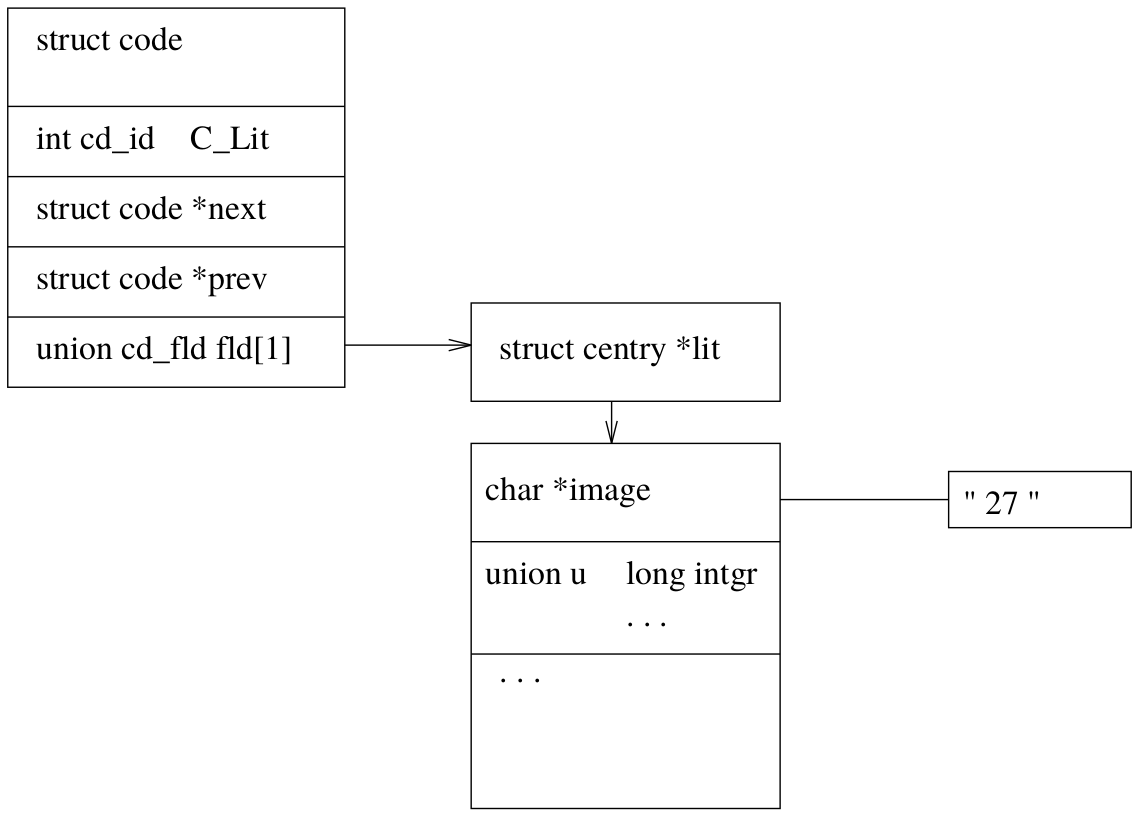
\includegraphics[width=6.0in,height=4.0in]{struct_code_literal.png}

Figure 25-5: Literal
\end{center}


Once the analysis is complete and the literal table is built then the
function \texttt{propagate\_literals} is called which goes through
each entry in the literal table and examines the code beginning at the
\texttt{initial} field until the \texttt{struct code} referenced by
the \texttt{end} field is encountered. If a \texttt{struct code} is
found that references the descriptor containing the current literal
then that reference is replaced by the literal itself. Figure 25-2
showed a fragment of code for generating an assignment, and Figure
25-6 shows the same fragment with the second descriptor replaced with
its literal (assuming that descriptor location 8 was previously
initialized to 27). It is important to note that only the
\texttt{struct val\_loc} on the right side of the equal sign will be
replaced by its literal.


\bigskip

\begin{center}
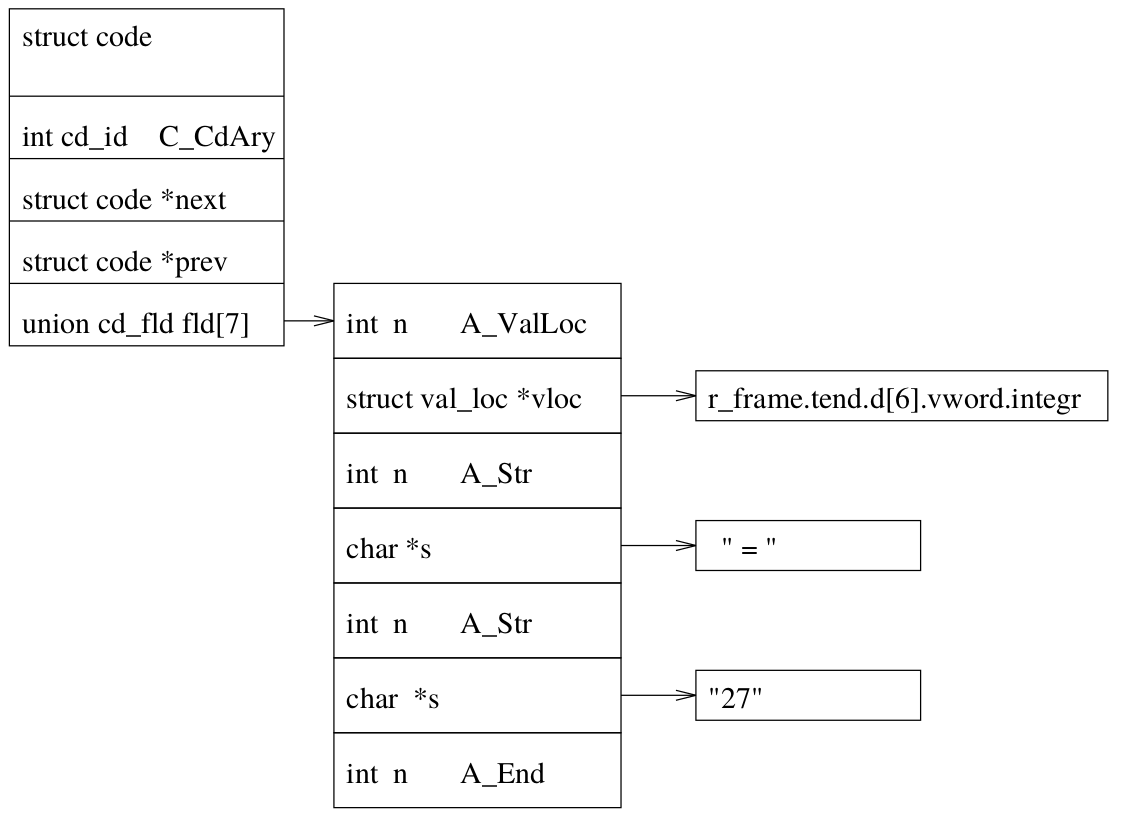
\includegraphics[width=6.0in,height=4.0in]{struct_code_assign_prop.png}

Figure 25-6: After Assignment
\end{center}


\subsection{New Functions}

The following functions were created to support the constant
propagation optimization. All these functions are placed in the
compiler source file \textfn{ccode.c}. Each function used in the
constant propagation is prototyped and described below.

\iconline{ struct lit\_tbl *alc\_tbl(void) }

This function allocates a \texttt{struct lit\_tbl} entry that contains
information about a literal and its usage. It first checks a global
pointer called \texttt{free\_lit\_tbl} to see if there are any free
table structures that may be reused. If there are no free structures
in this list then a new structure is allocated. Lastly, the fields are
initialized to predefined values.

\iconline{ novalue free\_tbl(void) }

This function frees the memory used for the current table by attaching
the current table to the list of free table structures
(\texttt{free\_lit\_tbl}).

\iconline{ novalue tbl\_add(struct lit\_tbl *add) }

This function adds a new \texttt{struct lit\_tbl} structure into the current
table. The insertion is to the end of the table plus it checks for the
previous use of the descriptor location used in the element being
added. For the previous use of the same element, that location's
\texttt{end} pointer is set to the initial pointer of the element
being added. In essence, this defines a scope for each descriptor
location. Once \texttt{end} is set for the first time, it should not
be changed later.

\iconline{ int substr(const char *str, const char *sub) }

This function is used to scan strings for logical operators
(\texttt{==}, \texttt{!=}, \texttt{{\textgreater}=},
\texttt{{\textless}=}, etc). If the string represented by \texttt{sub}
is found in \texttt{str} then \texttt{TRUE} is returned. It is
necessary to identify these operators so a string is not propagated as
an operand to one of these operators which is not valid C syntax.

\iconline{ int instr(const char *str, int chr) }

This function is used to determine if a string contains an assignment
operator. \ This function will return \texttt{TRUE} if the string
\texttt{str} contains any type of assignment (\texttt{=}, \texttt{+=},
\texttt{{}-=}, \texttt{*=}, \texttt{/=}, or \texttt{\%=}).

\iconline{ novalue invalidate(struct val\_loc *v, struct code *end, int code) }


This function sets values for an element in the literal table. For all
literal table entries that point to the \texttt{struct val\_loc}
represented by \texttt{v} the \texttt{end} field is set to
\texttt{end} with the \texttt{modified} field set to
\texttt{code}. \texttt{code} can be one of the following enumerated
values: \texttt{NO\_LIMIT}, \texttt{LIMITED},
\texttt{LIMITED\_TO\_INT}, or \texttt{NO\_TOUCH}.

\iconline{ novalue analyze\_literals(struct code *start, struct code *top, int lvl) }


This function steps through the \texttt{struct code} list for each
function, building up a literal table, and analyzing the scope between
which each literal can be safely propagated. It checks for loop
control variables, when and if the value of a constant descriptor
location changes, and checks to see if a descriptor location is passed
by reference to any functions.

\iconline{ novalue propagate\_literals(void) }

This function steps through each entry in the literal table and begins
to replace occurences of the descriptor location with the literal
between the \texttt{struct code} structures from the \texttt{initial}
field to the \texttt{end} field.  The function \texttt{eval\_code} is
called to do the actual propagation.

\iconline{ int eval\_code(struct code *cd, struct lit\_tbl *cur) }

This function first checks to see if the descriptor index of the code
currently being examined matches that of the current literal table
entry. If the current descriptor is accessed as an integer or a string
then the descriptor is replaced with the literal value. Also, the
\texttt{modified} is checked to see if there are any restrictions on
replacement. The table in Figure 25-7 lists the restrictions for
each possible value of \texttt{modified}.

\begin{center}
\tablefirsthead{\hline
{\itshape Name} &
{\itshape Replacement Restrictions}\\}
\tablehead{\hline
{\itshape Name} &
{\itshape Replacement Restrictions}\\}
\tabletail{}
\tablelasttail{}
\begin{xtabular}{|m{1.4670599in}|m{3.2670598in}|}
\hline
{\ttfamily NO\_LIMIT} &
 Always replace\\\hline
{\ttfamily LIMITED} &
 Always replace within \texttt{initial} and \texttt{end}\\\hline
{\ttfamily LIMITED\_TO\_INT} &
 Only replace if used as int, also limited by scope\\\hline
{\ttfamily NO\_TOUCH} &
 Never replace\\\hline
\end{xtabular}
\end{center}
{\centering\selectlanguage{english}
Figure 25-7: Replacement Policy
\par}


The actual replacement of a descriptor reference to a literal is
accomplished by setting the current index into the \texttt{fld} array
to the \texttt{A\_Str} type and allocating a string where the literal
is copied into. Figure 25-2 and Figure 25-6 illustrate an occurrence
of this.

\section{Variable Initialization}

Another issue is the initialization of the descriptor tables in each C
function that is generated by the Icon compiler.  Many of the
generated functions contain a loop that initializes all the entries of
the local descriptor table to the null descriptor. This is rather
cumbersome and generates a great deal of overhead.


\subsection{Eliminating Dead Code}

The first optimization to the variable initialization was to eliminate
``dead'' code, which is code that is never executed. In some cases the
loops that initialize the descriptor tables resembled this:

\goodbreak
\begin{iconcode}
for (i = 0; i < 0; ++i)\\
\>r\_frame.tend.d[i] = nulldesc;\\
\end{iconcode}


This code is generated for Icon library functions in the function
\texttt{outerfnc} located in \textfn{codegen.c}. There is a separate
function that outputs similar code for user written functions which
does check to see if the loop will ever execute. Both functions
contain a variable \texttt{ntend} which hold the number of descriptor
entries. A simple check for equality with zero was added.

\subsection{Loop Unrolling}

Every user function initializes all tended descriptor entries to the
value of the null descriptor \texttt{nulldesc} at the beginning of the
function. It is a simple one-line \texttt{for} loop similar to the
following code fragment.

\goodbreak
\begin{iconcode}
for (i = 0; i < 3; ++i)\\
\>r\_frame.tend.d[i] = nulldesc;\\
\end{iconcode}


Also, upon examining the C code generated from several programs, the
number of descriptor entries per procedure rarely exceeds ten. Because
this is a relatively small number, these loops can be unrolled into a
series of assignments, and the loop may be removed. The following code
is the above loop unrolled.

\goodbreak
\begin{iconcode}
r\_frame.tend.d[0] = nulldesc;\\
r\_frame.tend.d[1] = nulldesc;\\
r\_frame.tend.d[2] = nulldesc;\\
\end{iconcode}

While this will increase the size of the generated code, the loop
overhead is eliminated. There is a limit placed on the number of loop
iterations that will be unrolled which is defined in
\textfn{define.h}. Currently, this value, \texttt{LoopThreshold}, is
set to 6. Because this number and the number of descriptor table
entries is small, the number of unrolled elements is reasonable, and
the code size is not greatly affected.


The code that unrolls these loops is in the function \texttt{outerfnc}
in the file \textfn{codegen.c}. Because this change is only several
lines, the code that implements loop unrolling is included below.

\goodbreak
\begin{iconcode}
\#ifdef OptimizeLoop\\
\> if (ntend > 0) \ \ \ \ \ \ \ \ \ \ /* Check for dead code */\\
\> \>for (i=0; i < ntend ;i++)\\
\> \>\>fprintf(codefile,\\
\> \>\>\>\>\ \ " \ \ r\_frame.tend.d[\%d] = nulldesc; {\textbackslash}n",i);\\
\#else\\
\> fprintf(codefile, "for (i=0; i < \%d ;i++) {\textbackslash}n", ntend);\\
\> fprintf(codefile, " \ \ f\_frame.tend.d[i] = nulldesc;{\textbackslash}n;");\\
\#endif\\
\end{iconcode}

\section{Results}

Several tests were run to determine whether the code generation
optimizations were effective. These optimizations were performed in
hopes of improving the execution speed of the compiled program,
reducing the size of the intermediate code and the resulting
executable, and the compilation time.

Overall, the optimizations improved the execution speed by a modest
amount. The improvement is roughly between 6-8.25\%.  While this is
not a great as was hoped, it still is an improvement. The code size of
both the intermediate code and the generated executable are
suprisingly smaller. The loop unrolling seemed to be offset by the
constant progagation which eliminated unnecessary assigments and
references. The size of the executables were reduced by approximately
4-8\% for large programs, but there was no change in executable size
for small programs (20 lines). The size of the generated C file was
consistently around 3\% smaller than before the optimizations.
Also, on average around half of all calls to \texttt{Poll()} were
removed, and in one case, two thirds were eliminated.

The rest of this section presents detailed information on the results of the
optimizations for removing redundant function calls, unrolling loops,
removing dead code, and propagating literals.  Details of the results
of the code generation optimizations are presented in the areas of
execution speed, code size, and compilation time. These tests were run
on several programs. The first program, \textit{Beards}, generates
production grammars, non-terminals, terminals, and epsilon sets from
an input grammar. The second program, \textit{Yhcheng}, is a line
editor similar to \texttt{ed} which also has revision control
capabilities. For the code size and compilation time tests, two other
programs, \textit{Ctree} and \textit{Sphere}, were used for
tests. \textit{Beards}, \textit{Yhcheng}, and \textit{Ctree} are all
large programs while \textit{Sphere} is included because it is a very
small program (less than 25 lines).  All timings performed used the
Unix or Linux \texttt{time} utility.  Also note that these timings
were performed with all optimizations turned on including the type
representation optimization.

\subsection{Execution Speed}

Each program was run 10 times with sample input and averages were
computed. Figure 25-8 summarizes the execution times for
\textit{Beards} and \textit{Yhcheng}.

\begin{center}
\tablefirsthead{\hline
{\itshape Program} &
{\itshape Version} &
{\itshape User} &
{\itshape System} &
{\itshape Elapsed}\\}
\tablehead{\hline
{\itshape Program} &
{\itshape Version} &
{\itshape User} &
{\itshape System} &
{\itshape Elapsed}\\}
\tabletail{}
\tablelasttail{}
\begin{xtabular}{|m{1.1212599in}|m{1.1212599in}|m{1.1212599in}|m{1.1212599in}|m{1.1212599in}|}
\hline
~
 &
 Optimized &
\raggedleft 0.5 &
\raggedleft 0.12 &
\raggedleft\arraybslash 00:01.17\\\hline
 Beards &
 Unoptimized &
\raggedleft 0.52 &
\raggedleft 0.13 &
\raggedleft\arraybslash 00:01.27\\\hline
~
 &
 Improvement &
\raggedleft 4.97\% &
\raggedleft 9.09\% &
\raggedleft\arraybslash 8.25\%\\\hline
~
 &
 Optimized &
\raggedleft 0.59 &
\raggedleft 1.11 &
\raggedleft\arraybslash 00:01.99\\\hline
 Yhcheng &
 Unoptimized &
\raggedleft 0.62 &
\raggedleft 1.27 &
\raggedleft\arraybslash 00:02.14\\\hline
~
 &
 Improvement &
\raggedleft 4.21\% &
\raggedleft 12.91\% &
\raggedleft\arraybslash 6.79\%\\\hline
\end{xtabular}
\end{center}
{\centering\selectlanguage{english}
Figure 25-8: Execution Times
\par}

\subsection{Code Size}

Tests were run on the same two programs to determine if there was an
improvement in either the intermediate code size or the size of the
resulting executable. Figure 25-9 displays the code sizes for
\textit{Beards}, \textit{Yhcheng}, \textit{Ctree}, and
\textit{Sphere}. The first three programs are large (500-1800 lines)
while \textit{Sphere} is small (20 lines).

\begin{center}
\tablefirsthead{\hline
{\itshape Program} &
{\itshape Version} &
{\itshape C File} &
{\itshape H File} &
{\itshape Executable}\\}
\tablehead{\hline
{\itshape Program} &
{\itshape Version} &
{\itshape C File} &
{\itshape H File} &
{\itshape Executable}\\}
\tabletail{}
\tablelasttail{}
\begin{xtabular}{|m{1.1212599in}|m{1.1212599in}|m{1.1212599in}|m{1.1212599in}|m{1.1212599in}|}
\hline
~
 &
 Optimized &
\raggedleft 246159 &
\raggedleft 12967 &
\raggedleft\arraybslash 204800\\\hline
 Beards &
 Unoptimized &
\raggedleft 252041 &
\raggedleft 12967 &
\raggedleft\arraybslash 212992\\\hline
~
 &
 Improvement &
\raggedleft{\itshape 2.33\%} &
\raggedleft{\itshape 0.00\%} &
\raggedleft\arraybslash{\itshape 3.85\%}\\\hline
~
 &
 Optimized &
\raggedleft 554014 &
\raggedleft 46168 &
\raggedleft\arraybslash 294912\\\hline
 Yhcheng &
 Unoptimized &
\raggedleft 568118 &
\raggedleft 46168 &
\raggedleft\arraybslash 319488\\\hline
~
 &
 Improvement &
\raggedleft{\itshape 2.48\%} &
\raggedleft{\itshape 0.00\%} &
\raggedleft\arraybslash{\itshape 7.70\%}\\\hline
~
 &
 Optimized &
\raggedleft 290536 &
\raggedleft 61545 &
\raggedleft\arraybslash 225280\\\hline
 Ctree &
 Unoptimized &
\raggedleft 298813 &
\raggedleft 61545 &
\raggedleft\arraybslash 237568\\\hline
~
 &
 Improvement &
\raggedleft{\itshape 2.77\%} &
\raggedleft{\itshape 0.00\%} &
\raggedleft\arraybslash{\itshape 5.17\%}\\\hline
~
 &
 Optimized &
\raggedleft 82289 &
\raggedleft 49755 &
\raggedleft\arraybslash 159744\\\hline
 Sphere &
 Unoptimized &
\raggedleft 84972 &
\raggedleft 49755 &
\raggedleft\arraybslash 159744\\\hline
~
 &
 Improvement &
\raggedleft{\itshape 3.16\%} &
\raggedleft{\itshape 0.00\%} &
\raggedleft\arraybslash{\itshape 0.00\%}\\\hline
\end{xtabular}
\end{center}
{\centering\selectlanguage{english}
Figure 25-9: Code Sizes
\par}


Much of the reduction in code size can be attributed to the removal of
redundant calls to \texttt{Poll}, and it is this reduction that
offsets the loop unrolling. Improvements on \textit{Beards},
\textit{Yhcheng}, and \textit{Sphere} show that almost one half of all
calls to \texttt{Poll} were eliminated; however, \textit{Ctree} shows
almost a two thirds reduction. Figure 25-10 shows the number of calls
to \texttt{Poll} for each program before and after the optimization.

\begin{center}
\tablefirsthead{\hline
{\itshape Test Program} &
 No. Before &
 No. After\\}
\tablehead{\hline
{\itshape Test Program} &
 No. Before &
 No. After\\}
\tabletail{}
\tablelasttail{}
\begin{xtabular}{|m{0.9406598in}|m{0.76435983in}|m{0.6712598in}|}
\hline
 Beards &
\raggedleft 810 &
\raggedleft\arraybslash 481\\\hline
 Yhcheng &
\raggedleft 2144 &
\raggedleft\arraybslash 1135\\\hline
 Ctree &
\raggedleft 745 &
\raggedleft\arraybslash 293\\\hline
 Sphere &
\raggedleft 40 &
\raggedleft\arraybslash 22\\\hline
\end{xtabular}
\end{center}
{\centering\selectlanguage{english}
Figure 25-10: Number of Redundant Functions Removed
\par}

{\sffamily
Compilation Time}

Lastly, the compilation times for the sample programs are given. Each
program was compiled five times with the results averaged. Again,
results for the \textit{Beards}, \textit{Yhcheng}, \textit{Ctree}, and
\textit{Sphere} are in Figure 25-11.

\begin{center}
\tablefirsthead{\hline
{\itshape Program} &
{\itshape Version} &
{\itshape User} &
{\itshape System} &
{\itshape Elapsed}\\}
\tablehead{\hline
{\itshape Program} &
{\itshape Version} &
{\itshape User} &
{\itshape System} &
{\itshape Elapsed}\\}
\tabletail{}
\tablelasttail{}
\begin{xtabular}{|m{0.6288598in}|m{0.9636598in}|m{0.5997598in}|m{0.54205984in}|m{0.6420598in}|}
\hline
~
 &
 Optimized &
\raggedleft 43.57 &
\raggedleft 1.77 &
\raggedleft\arraybslash 00:47.40\\\hline
 Beards &
 Unoptimized &
\raggedleft 60.93 &
\raggedleft 1.65 &
\raggedleft\arraybslash 01:02.93\\\hline
~
 &
 Improvement &
\raggedleft{\itshape 28.49\%} &
\raggedleft{\itshape {}-7.27\%} &
\raggedleft\arraybslash{\itshape 24.68\%}\\\hline
~
 &
 Optimized &
\raggedleft 116.97 &
\raggedleft 2.76 &
\raggedleft\arraybslash 02:04.14\\\hline
 Yhcheng &
 Unoptimized &
\raggedleft 163.37 &
\raggedleft 2.86 &
\raggedleft\arraybslash 02:49.71\\\hline
~
 &
 Improvement &
\raggedleft{\itshape 28.40\%} &
\raggedleft{\itshape 3.50\%} &
\raggedleft\arraybslash{\itshape 26.85\%}\\\hline
~
 &
 Optimized &
\raggedleft 65.26 &
\raggedleft 2.54 &
\raggedleft\arraybslash 01:13.44\\\hline
 Ctree &
 Unoptimized &
\raggedleft 92.25 &
\raggedleft 2.88 &
\raggedleft\arraybslash 01:47.44\\\hline
~
 &
 Improvement &
\raggedleft{\itshape 29.26\%} &
\raggedleft{\itshape 11.81\%} &
\raggedleft\arraybslash{\itshape 31.65\%}\\\hline
~
 &
 Optimized &
\raggedleft 11.98 &
\raggedleft 1.83 &
\raggedleft\arraybslash 00:16.36\\\hline
 Sphere &
 Unoptimized &
\raggedleft 13.62 &
\raggedleft 2.22 &
\raggedleft\arraybslash 00:18.85\\\hline
~
 &
 Improvement &
\raggedleft{\itshape 12.04\%} &
\raggedleft{\itshape 17.57\%} &
\raggedleft\arraybslash{\itshape 13.21\%}\\\hline
\end{xtabular}
\end{center}
{\centering\selectlanguage{english}
Figure 25-11: Compile Times
\par}

\subsection{Analysis of Intermediate Code Optimizations}

The gains in execution speed and code size were modest but not
startling. For the most part, improvement was less than 10\%.
However, the results for compilation time are more promising. The
speedup was between 24\% and 31\% for large programs, which is between
a 15 and 45 second improvement.

The eliminated functions calls most likely have a negligible effect on
execution speed but greatly contributed to the reduction in code
size. For example, on a large program like \textit{Yhcheng} which
contained more than 18,600 lines of C code, approximately 450
redundant calls were removed. It was not expected that eliminating
{\textasciigrave}{\textasciigrave}dead'{}' initialization loop would
have much effect on execution speed. Constant propagation and loop
unrolling probably accounted for the improved execution
times. However, more of an improvement was expected from the constant
propagation optimization. Two possible explanations could be that the
native C compiler is able to reduce the complex structure lookup to
its literal value or that the compiler has so much other baggage
slowing down execution that the constant propagation improvement was
not enough to make a great difference. The second explanation seems
more likely.

The size of the intermediate code and executable code were also
modestly improved. The elimination of redundant function calls offset
the addition of code due to loop unrolling. Also, eliminating
unnecessary initializations for literals that were propagated
contributed to the smaller code sizes. It is important to note that as
it is, the compiler generates an enormous amount of code for procedure
continuations and suspensions so that 25-30\% of the intermediate code
are these functions and the rest is user code.

Lastly, the speed of compilation was a pleasant surprise; however, I
do believe that this improvement is due to the type inferencing
optimization because the current optimizations being discussed only
add extra logic to improve the generated code. Another significant
factor is that less memory is being used by the type inferencing
system, which therefore causes less access to virtual memory. I should
note that all the tests were run with that optimization on, and the
improvement to type inferencing simplifies the type system in many
ways. To determine if a specific bit is set, the old system had to
create a mask and find the appropriate index into a long bit
vector. The new system requires a single comparison in the case of the
five builtin types.

\section{Conclusion and Future Optimizations}

All of the optimizations discussed in this chapter have been
implemented. Some of the optimizations performed extremely well while
others did not have much effect. The type representation change
provided a substantial improvement on the memory usage required by the
type inferencing system. As was stated early, the compiler still uses
too much memory to be of much use to the average Icon programmer but
is much better suited to offering the added speedup of compiled code
when occasionally necessary.

The intermediate code optimizations were really just the tip of the
iceberg of all the possible improvements to this area. The removal of
redundant calls to system calls was a small improvement. Literal
propagation was probably the most significant improvement along with
loop unrolling. Further optimizations in this area are likely to yield
the best improvements to performance.

After studying the generated code, several other optimizations were
identified that may offer additional improvements to both the speed of
execution and the size of the intermediate and executable code. The
next few paragraphs describe additional optimizations and are
organized in the order of the easiest to hardest to implement.

\liststyleLxxxvi
\begin{enumerate}
\item 
For the unrolled descriptor initializations change the indexing array to pointer arithmetic which is faster. For example
the following code fragment is modified as follows: 
\end{enumerate}
\goodbreak
\begin{iconcode}
r\_frame.tend.d[0] = nulldesc;\\
r\_frame.tend.d[1] = nulldesc;\\
r\_frame.tend.d[2] = nulldesc;\\
\end{iconcode}
\goodbreak
\makebox[0.5\textwidth]{\hrulefill}
\begin{iconcode}
register dptr p;\\
p = r\_frame.tend.d;\\
(p++)->dword = nulldesc;\\
(p++)->dword = nulldesc;\\
\end{iconcode}

\liststyleLxxxvii
\begin{enumerate}
\item 
Analyze the logic of loops and also unroll smaller ones. For example,
the following loop appears at the beginning of most functions.
\end{enumerate}
\goodbreak
\begin{iconcode}
for (i = 0; i < r\_nargs ; ++i)\\
\>deref(\&r\_args[i], \&r\_frame.tend.d[i + 0]);\\
for(i = r\_nargs; i < 2 ; ++i)\\
\>r\_frame.tend.d[i + 0] = nulldesc;\\
\end{iconcode}


In this case \texttt{r\_nargs} cannot be greater than two because it
was earlier declared to have only two entries. It would be necessary
to guarantee that \texttt{r\_nargs} can never be more than two, but if
it is certain that there are exactly two elements then we can write
the initialization loop as follows:

\goodbreak
\begin{iconcode}
if(r\_nargs > 0) \{\\
\>deref(\&r\_args[0], \&r\_frame.tend.d[0]);\\
\>if (r\_nargs > 1)\\
\>\>deref(\&r\_args[1], \&r\_frame.tend.d[1]);\\
\>else\\
\>\>tend.d[1].dword = D\_Null;\\
\>\}\\
else\\
\>tend.d[0].dword = D\_Null;\\
\end{iconcode}


This optimization could lead to a gain in execution speed. For
example, if the unrolling is performed on descriptors with array sizes
of one or two, approximately 40\% of these loops would be unrolled.

\liststyleLxxxviii
\begin{enumerate}

\item An easy and obvious solution would be to simplify expressions like
\texttt{i + 0} which commonly occur. This will not improve execution
time because the C compiler will catch this, but by removing it before
writing the statement to the intermediate file, the compile time of
the C compiler will be improved.

\item Another easy optimization would be to shorten variable
names. This causes a penalty by having to write long names such as
\texttt{r\_frame.tend.d} to file and then having the C compiler read
it back in. This could be changed to \texttt{r\_f.t.d}. While this
makes the intermediate C code hard to read, the intermediate code is
not meant to be inspected by the user and will result in faster
compilations.

\item For the initialization loops present in all functions, remove the
initialization of the loop control variable when unnecessary. Consider
the following loop:
\end{enumerate}
\goodbreak
\begin{iconcode}
for (i = 0; i < r\_nargs ; ++i)\\
\>deref(\&r\_args[i], \&r\_frame.tend.d[i + 0]);\\
for(i = r\_nargs; i < 2 ; ++i)\\
\>r\_frame.tend.d[i + 0] = nulldesc;\\
\end{iconcode}


The variable \texttt{i} in the second loop does not need to be
initialized since it is already at the value that it is supposed to be
for the second loop. The next fragment of code illustrates this change.

\goodbreak
\begin{iconcode}
for (i = 0; i < r\_nargs ; ++i)\\
\>deref(\&r\_args[i], \&r\_frame.tend.d[i + 0]);\\
for( ; i < 2 ; ++i)\\
\>r\_frame.tend.d[i + 0] = nulldesc;\\
\end{iconcode}


While this change is very easy, it is questionable whether this will
provide noticeable improvement in execution except in large programs
where these loops are very common.

\liststyleLxxxix
\begin{enumerate}
\item 
\ Assignments of the \texttt{r\_frame.tend.d} structures may be simplified. Consider the following assignment:
\end{enumerate}
\goodbreak
\begin{iconcode}
r\_frame.tend.d[2] /* i */.vword.integr =\\
\>r\_frame.tend.d[4].vword.integr;\\
r\_frame.tend.d[2] /* i */.dword = D\_Integer;\\
\end{iconcode}


This could be changed into a single assignment as follows:

\iconline{ \ \ r\_frame.tend.d[2] = r\_frame.tend.d[4]; }


This optimization would require more work than the previously
described ones. Each \texttt{struct val\_loc} structure would have
to be examined, including the context in which it is used in order to
catch assignments such as this; however, these assignments are very
common and could lead to substantial gains in execution speed.

\liststyleLxl
\begin{enumerate}
\item 
\ Similarly, perform the same simplified descriptor assignment on global descriptor locations. A method needs to be
created for changing global assignments such as:
\end{enumerate}
\goodbreak
\begin{iconcode}
globals[63] /* rnode */.dword = D\_Integer;\\
globals[63] /* rnode */.vword.integr = 1;\\
\end{iconcode}

\noindent
into

\iconline{globals[63] /* rnode */ = onedesc; }

\noindent where \texttt{onedesc} is a single descriptor that already
contains the values of the \texttt{dword} and \texttt{vword} being
assigned. This could be performed by creating several constant
decriptors for the common values such as 0 or 1.  Like the previous
optimization, this change will offer a smaller improvement to
execution speed because global descriptor assignments occur much less
frequently.

\liststyleLxli
\begin{enumerate}
\item 
When a variable is dereferenced, it is often the case that the
variable location is passed in for both parameters to the
\texttt{deref} function. For example, in the following code example,
\texttt{r\_frame.tend.d[7]} is the variable being derefenced and the
location where the dereferenced value is to be placed. This can be
simplified by creating another version of \texttt{deref}, perhaps
named \texttt{deref1}, that takes a single argument, dereferences it,
and places the dereferenced value into the parameter location.
\end{enumerate}
\iconline{deref(\&r\_frame.tend.d[7], \&r\_frame.tend.d[7]); }

\liststyleLxlii
\begin{enumerate}
\item 
Another issue is redundant constant initializations. Consider the following code:
\end{enumerate}
\goodbreak
\begin{iconcode}
r\_frame.tend.d[8].dword = D\_Integer;\\
r\_frame.tend.d[8].vword.integr = 1;\\
if (!(argp[1] /* level */.vword.integr== 1) )\\
\>goto L19 /* bound */;\\
r\_frame.tend.d[8].dword = D\_Integer;\\
r\_frame.tend.d[8].vword.integr = 1;\\
\end{iconcode}


The descriptor location 8 is assigned the value of 1 and then a
conditional statement is performed which is followed by a possible
\texttt{goto}. If the jump does not occur then the same descriptor
location is assigned the same value over again. Clearly the second
assignment is wasteful and needs to be eliminated. This would
require fairly aggressive analysis of the intermediate code in order
to catch these code sequences, but does offer the benefits of
increased execution speed and smaller code size.


A more difficult optimization that offers a substantial reduction in
the size of the intermediate and executable code deals with the
initialization functions that set up frames. In the case of
\textit{Ctree}, over 30\% of the generated C code consists of these
functions. For example, in \textit{Ctree} there are two functions
named \texttt{P06i\_set\_value\_Vtext} and
\texttt{P03n\_unset\_Vbool\_coupler} which are identical except for
their frame structures, similarly defined as
\texttt{PF06i\_set\_value\_Vtext} and
\texttt{PF03n\_unset\_Vbool\_coupler}; however, these structures are
identical. A possible solution would be to write out one copy of each
unique frame structure along with its corresponding function that
would initialize that frame. In addition to the reduction of code size
this would result in faster compilations and faster loading of the
resulting executable. This last optimizations is the most difficult
and would require extensive changes; however, this optimization offers
the best improvements in code size, execution time, and compile time.
